\part{Funzioni e Successioni}
\section{Corrispondenze}
Siano\marginnote{5 ott 2021} $ X, Y $ insiemi, e consideriamo $ P(x,y) $ predicato su $ x \in X $ e su $ y \in Y $.
\esempi{}{
    \begin{itemize}
        \item $X$: fantini di una squadra\\ $Y$: cavalli della stessa squadra\\ $ P(x,y) $: $ x $ ha cavalcato almeno una volta $ y $;
        \item $ X=Y= \R $; $ P(x,y) $: $ x^{2}+y^{2}=1 $;
        \item $ X=Y= \R $; $ P(x,y) $: $ y=x^{2} $.
    \end{itemize}
}

\definizione{}{Una \textit{corrispondenza} $ \mathfrak{F} $ tra gli elementi di $ X $ e di $ Y $ è un predicato binario $ P(x,y) $ nelle variabili $ x \in X $, $ y \in Y $.

Diciamo che $ x \in X $ è in corrispondenza con $ y \in Y $ se $ P(x,y) $ è verificata. Scriviamo \[
    y=\mathfrak{F} (x)
\]}

\definizione{}{
    Sia $ \mathcal{R}  $ il \textit{sottoinsieme} di $ X\times Y $ costituito dalle coppie $(x,y)$ per cui la relazione è vera \[
        \mathcal{R} =\{(x,y) \in X\times Y\,|\, P(x,y)\text{ è verificata}\} \subseteq X\times Y
    \]
    $ \mathfrak{F}  $ è univocamente determinata da $ \mathcal{R}  $.

    $ \mathcal{R}  $ prende il nome di \textit{grafo} (o grafico) di $ \mathfrak{F}  $. Una corrispondenza è totalmente individuata dal grafo.
}

\esempio{}{
    $ X=Y= \R $, \begin{align*}
        \mathfrak{F}:\R & \to \R \\
    x & \mapsto y=\mathfrak{F}(x)\quad\text{ se } x^{2}+y^{2}=1
    \end{align*} \[
        \mathcal{R} =\{(x,y) \in \R^{2}\,|\, x^{2}+y^{2}=1\}
    \]
    \begin{center}
    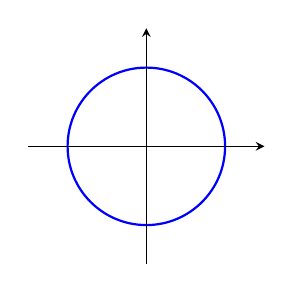
\begin{tikzpicture}
        \draw [blue, thick] (0,0) circle (1);
        \draw [-stealth] (-1.5, 0) -- (1.5, 0);
        \draw [-stealth] (0, -1.5) -- (0, 1.5);
    \end{tikzpicture}
    \end{center}
}
\begin{minipage}{\textwidth}
    \osservazione{
    Si noti come in questo esempio, 

    \vspace{0.5em}
    \begin{multicols}{2}
        \begin{align*}
        \frac{1}{2}&\to \frac{\sqrt{3}}{2}\\
        \frac{1}{2}&\to \frac{-\sqrt{3}}{2}
        \end{align*}
    \begin{center}
        \columnbreak

        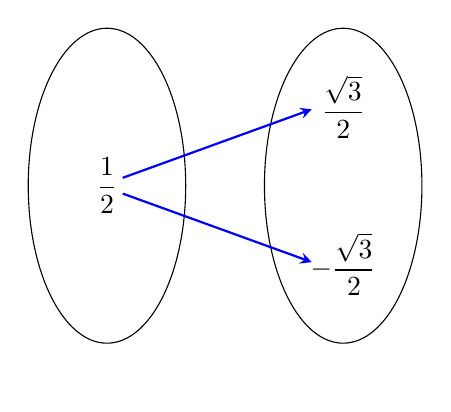
\begin{tikzpicture}
            \draw (-1.5,0) ellipse (1 and 2);
            \draw (1.5,0) ellipse (1 and 2);
            \node at (-1.5, -2.4) {$\R$};
            \node at (1.5, -2.4) {$\R$};
            \node at (-1.5, 0) {$\displaystyle%
            \frac{1}{2}$};
            \node at (1.5, 1) {$\displaystyle%
            \frac{\sqrt{3}}{2}$};
            \node at (1.5, -1) {$\displaystyle%
            -\frac{\sqrt{3}}{2}$};
            \draw [blue, thick, -stealth] (-1.3, 0.1) -- (1.1, 0.97); 
            \draw [blue, thick, -stealth] (-1.3, -0.1) -- (1.1, -0.97); 
        \end{tikzpicture}
    \end{center}
    \end{multicols}
    Mentre in altri casi, come \begin{align*}
    \mathscr{G} :\R & \to \R \\
    x & \mapsto x^{2}
    \end{align*} con \[
        \mathcal{R} =\{(x,y) \in \R^{2}\,|\, y=x^{2}\}
    \] vale \begin{equation}
        \forall\, x \in X=\R\quad \exists!\, y \in Y=\R\,\tc\, y=\mathscr{G} (x)\label{proprieta1}
    \end{equation}
}
\end{minipage}

\esempio{
    Sia $ X $ l'insieme dei fantini e $ Y $ l'insieme dei cavalli. $ Y= \mathscr{L}(x) $ se $ x  $ ha cavalcato almeno una volta $ y $. La corrispondenza può avere una forma simile:
    \begin{center}
        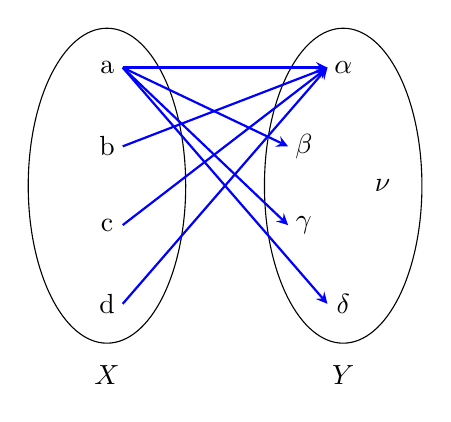
\begin{tikzpicture}
            \draw (-1.5,0) ellipse (1 and 2);
            \draw (1.5,0) ellipse (1 and 2);
            \node at (-1.5, -2.4) {$X$};
            \node at (1.5, -2.4) {$Y$};
            \node at (-1.5, 1.5) {a};
            \node at (-1.5, 0.5) {b};
            \node at (-1.5, -0.5) {c};
            \node at (-1.5, -1.5) {d};
            \node at (1.5, 1.5) {$\alpha$};
            \node at (1, 0.5) {$\beta$};
            \node at (1, -0.5) {$\gamma$};
            \node at (1.5, -1.5) {$\delta$};
            \node at (2, 0) {$\nu$};
            \draw [blue, thick, -stealth] (-1.3, 1.5) -- (1.3, 1.5); 
            \draw [blue, thick, -stealth] (-1.3, 1.5) -- (0.8, 0.5); 
            \draw [blue, thick, -stealth] (-1.3, 1.5) -- (0.8, -0.5); 
            \draw [blue, thick, -stealth] (-1.3, 1.5) -- (1.3, -1.5); 
            \draw [blue, thick, -stealth] (-1.3, 0.5) -- (1.3, 1.5); 
            \draw [blue, thick, -stealth] (-1.3, -0.5) -- (1.3, 1.5); 
            \draw [blue, thick, -stealth] (-1.3, -1.5) -- (1.3, 1.5); 
        \end{tikzpicture}
    \end{center}
    In questo caso la proprietà \eqref{proprieta1} non è soddisfatta.
}

Si nota che vi è una sostanziale differenza tra $ \mathscr{L} $ e $ \mathscr{G} $

\section{Funzioni}
\definizione{}{Una corrispondenza $ \mathscr{G} $:
    \begin{align*}
    \mathscr{G}: X & \to Y \\
     & x \mapsto y=\mathscr{G}(x)
    \end{align*} è una  textit{funzione} se $ \forall\,x \in X $ esiste al più un $ y \in Y $ tale che $ y=\mathscr{G}(x) $.
}

Nel corso si utilizzeranno sempre funzioni \begin{align*}
f:\R^{m} & \to \R^{n} \\
x & \mapsto y=f(x)
\end{align*}

\subsection{Definizioni}

\definizione{}{
    $ D \subseteq \R^{m} $ è detto \textit{dominio} di $ f $ se \[
        \forall\, x \in D\quad \exists\, y \in \R^{n}\,\tc\, y=f(x)
    \]

    Se non meglio specificato, $ D $ è dato da tutti gli $ x \in \R^{m} $ per cui l'espressione $ y =f(x) $ ha significato.
}
%DOMANDA: nella scrittura f:X\to Y, X è il dominio e Y è il codominio, vero? A questo punto, non è sbagliato scrivere log x: R\to R? Non andrebbe scritto log x: D\to R, specificando successivamente il dominio?
\definizione{}{Data una funzione \begin{align*}
f:X & \to Y \\
x & \mapsto y
\end{align*} si definisce \textit{codominio} di $ f $ l'insieme $ Y $.}
\esempio{}{
    $ f(x)=\ln (x-1) $, $ f: \R\to \R $. Deve valere $ x-1>0 $, pertanto \[
        D=(1, +\infty)=\{x \in \R\,|\, x>1\}
    \]
}
\notazione{}{
    Indichiamo \[
        D=\dom f
    \]
}
\esempio{}{
    Sia $ v=v(t) $ la velocità all'istante $ t $ di un corpo in caduta libera con velocità iniziale nulla.
    $ D \subseteq \R $ \begin{align*}
    v:D & \to \R \\
    t & \mapsto v(t)=g\,t
    \end{align*} con $ g $ accelerazione. Si noti che $ D\neq \R $, in quanto $ t $ è un tempo, e pertanto deve essere $ t\ge 0 $, allora \[
        D=[0, +\infty)=\{t \in \R; t\ge 0\}
    \]
}
\attenzione{Il dominio $ D=\dom f $ fa parte integrante della definizione della funzione, e deve essere sempre indicato.}
\esempio{}{\phantomsection\label{esempiofuncin}
        \begin{align*}
        f:\R &\to \R & g:[0; + \infty) &\to \R\\
        x & \mapsto y=x^{2} &  x &\mapsto y=x^{2}\\
        \dom f &= \R & \dom g &= [0; + \infty)
        \end{align*} 
        
        Si noti che \begin{align*}
            \graph (f)&=\{(x,y) \in \R\,|\, y=x^{2}\}\\ \graph (g)&=\{(x,y) \in [0; + \infty)\,|\, y=x^{2}\}
        \end{align*}

        $ f $ e $ g $ sono funzioni diverse.
}

\subsection{Funzioni iniettive, suriettive e biiettive}
\definizione{Data una funzione $ g:D\to Y $, $ f $ è \textit{iniettiva} se \begin{equation}
        \forall\,x_1, x_2 \in \dom g\qquad \begin{aligned}
            g(x_1)=g(x_2) \,&\implies\,x_1=x_2\\
            \big(x_1\neq x_2 \,&\implies\, g(x_1)\neq g(x_2)\big)
        \end{aligned}
    \end{equation}
}
\osservazione{}{
    La funzione $ g $ dell'\hyperref[esempiofuncin]{esempio (\thesection.\theesempi)} è iniettiva.
}
\definizione{}{
    Data $ f:D\to Y $, $ D=\dom f $, diciamo \textit{immagine} di $ f $ \begin{equation}
        f(D)=\im (f)=\bigl\{y \in Y\,\tc\quad \exists\, x \in D\,|\, y =f(x)\bigl\}
    \end{equation}
}
\definizione{}{
    Diciamo che \begin{align*}
    f:D & \to Y \\
    x & \mapsto f(x)
    \end{align*} è \textit{suriettiva} se \begin{equation}
        \forall\, y \in Y\quad \exists\, x \in D\,\tc\, y=f(x)
    \end{equation}
}

Una funzione $ f:D\to f(D) $ è sempre suriettiva.

\definizione{}{Diciamo che $ f: D\to Y $ è \textit{biettiva} (biunivoca) se è sia suriettiva che iniettiva.}

\subsection{Funzione composta}

Siano $ X, Y, W $ insiemi generici, e siano \begin{gather*}
    \begin{aligned}
        f: D &\to Y\\
        x &\mapsto y =f(x)
    \end{aligned}\qquad D=\dom f \subseteq X\\
    \begin{aligned}
        g: D' &\to w\\
        y &\mapsto w =g(x)
    \end{aligned}\qquad D'=\dom g \subseteq Y
\end{gather*}

Assumendo $ f(D) \subseteq D' $, possiamo costrure $ F $:
\begin{center}
    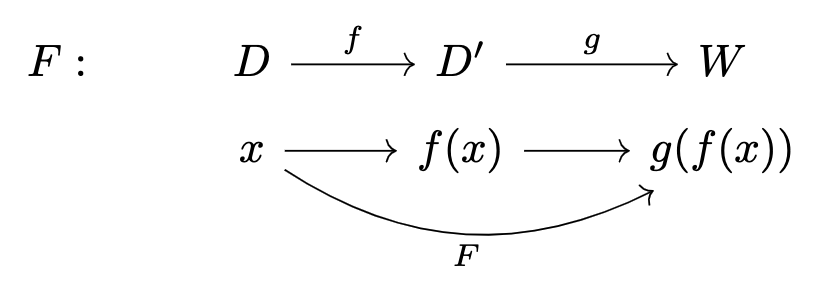
\includegraphics[width=7cm]{1.png}
\end{center}

La funzione \begin{align*}
F:D & \to W \\
x & \mapsto F(x)=g\bigl(f(x)\bigr)
\end{align*} è detta \textit{funzione composta} di $ f $ e $ g $. Si indica \[
    F=g\circ f
\]
\esempio{}{
    Siano $ D, D' \subseteq \R $, \[
        \begin{aligned}
            f: D&\to \R\\
            x &\mapsto x^{2}
        \end{aligned}\hspace{4em}\begin{aligned}
            g: D' &\to \R\\
            x&\mapsto \sqrt{x}
        \end{aligned}
    \]
    \vspace{1em}

    \begin{multicols}{2}
        \begin{center}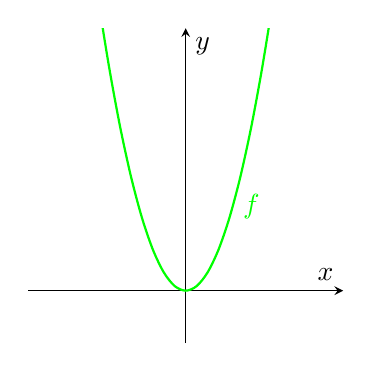
\begin{tikzpicture}\begin{axis}[
                xlabel=$x$,
                ylabel=$y$,
                axis equal,
                axis lines=middle,
                enlargelimits,
                xmax=5,
                xmin=-5,
                ymax=9,
                ymin=-1,
                xtick={0},
                ytick={0},
                scale only axis, 
                height=4cm, 
                width=4cm
                ]
            \addplot [no marks, green, smooth, thick, x=-1:5] {x^2};
            \node at (2.5, 3.2) {\textcolor{green}{$f$}};
        \end{axis}\end{tikzpicture}\end{center}
        \columnbreak

        \begin{center}
        \begin{tikzpicture}
            \begin{axis}[
                xlabel=$x$,
                ylabel=$y$,
                axis equal,
                axis lines=middle,
                enlargelimits,
                xmax=5,
                xmin=-1,
                ymax=5,
                ymin=-1,
                xtick={0},
                ytick={0},
                scale only axis, 
                height=4cm, 
                width=4cm
                ]
                \addplot [no marks, blue, smooth, thick, domain=0:5] {x^0.5};
                \node at (1, 1.6) {\textcolor{blue}{$g$}};
            \end{axis}
        \end{tikzpicture}\end{center}
    \end{multicols}
    

    Sia ha $ D=\dom f=\R $, $ D'=\dom g=[0, + \infty) $. Inoltre \[
        f(D)=[0, + \infty) \subseteq \dom g
    \] \begin{align*}
    g\circ f:\R & \to [0, + \infty) \\
    x & \mapsto \sqrt{x^{2}}=|x|
    \end{align*}

    Vale $ \dom f= \R $, $ \dom g=[0, + \infty) $, $ \dom (g\circ f)= \R $

    \begin{center}
    \begin{tikzpicture}
        \begin{axis}[
            xlabel=$x$,
            ylabel=$y$,
            axis equal,
            axis lines=middle,
            enlargelimits,
            xmax=5,
            xmin=-5,
            ymax=5,
            ymin=-1,
            xtick={0},
            ytick={0},
            scale only axis, 
            height=4cm, 
            width=6cm
            ]
            \addplot [no marks, red, smooth, thick, domain=-5:0] {-x};
            \addplot [no marks, red, smooth, thick, domain=0:5] {x};
            \node at (1, 2.3) {\textcolor{red}{$g\circ f$}};
        \end{axis}
    \end{tikzpicture}\end{center}
}   
\esempio{}{
    \[
        \begin{aligned}
            D& \subseteq \R^{2}\\
            f:D & \to \R^{2} \\
            x=(x_1,x_2) & \mapsto y=(x_1^{2},x_2^{2})
        \end{aligned}\qquad
        \begin{aligned}
            D'& \subseteq \R^{2}\\
            g:D' & \to \R \\
            x=(x_1,x_2) & \mapsto y=\sqrt{x_1+x_2}
        \end{aligned}
    \]
    Vale: $ D=\dom f=\R^{2} $ \[
        \im (f)=[0, + \infty)\times [0, + \infty)
    \]
    \begin{center}
        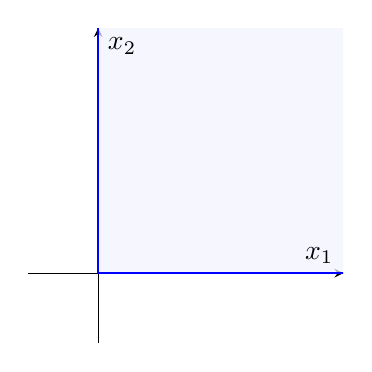
\begin{tikzpicture}
            \begin{axis}[
                xlabel=$x_1$,
                ylabel=$x_2$,
                axis equal,
                axis lines=middle,
                enlargelimits,
                xmax=5,
                xmin=-1,
                ymax=5,
                ymin=-1,
                xtick={0},
                ytick={0},
                scale only axis, 
                height=4cm, 
                width=4cm
                ]
                \addplot [no marks, blue, thick, fill=blue!5, fill opacity=0.7] coordinates {(0,0) (0,7) (7,7) (7, 0) (0,0)};
            \end{axis}
        \end{tikzpicture}\end{center}

        Inoltre \[
            D'=\dom g=\{(x_1, x_2) \in \R^{2}\,|\, x_1+x_2\ge 0\}
        \]
        \begin{center}
            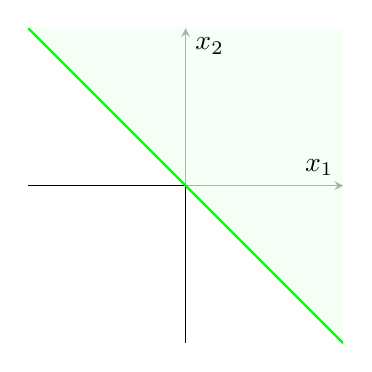
\begin{tikzpicture}
                \begin{axis}[
                    xlabel=$x_1$,
                    ylabel=$x_2$,
                    axis equal,
                    axis lines=middle,
                    enlargelimits,
                    xmax=5,
                    xmin=-5,
                    ymax=5,
                    ymin=-5,
                    xtick={0},
                    ytick={0},
                    scale only axis, 
                    height=4cm, 
                    width=4cm
                    ]
                    \addplot [no marks, green, thick, fill=green!5, fill opacity=0.7] coordinates {(-7,7) (7,-7) (7,7) (-7, 7)};
                \end{axis}
            \end{tikzpicture}\end{center}

            Quindi $ \im(f) \subseteq \dom g $ \begin{align*}
            g\circ f:\R^{2} & \to \R \\
            x=(x_1,x_2) & \mapsto \sqrt{x_1^{2}+x_2^{2}}=|x|
            \end{align*}
            \begin{center}
                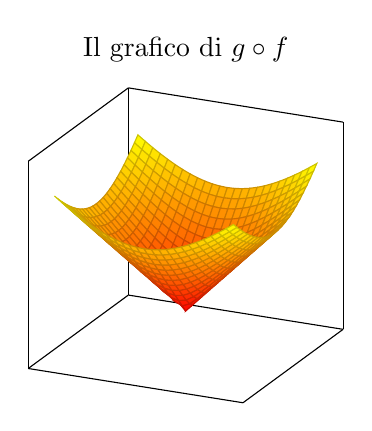
\begin{tikzpicture}
                    \begin{axis}[
                        xlabel=,
                        ylabel=,
                        zlabel=,
                        axis equal,
                        enlargelimits,
                        xmax=5,
                        xmin=-5,
                        ymax=5,
                        ymin=-5,
                        xtick=\empty,
                        ytick=\empty,
                        ztick=\empty,
                        scale only axis, 
                        height=4cm, 
                        width=4cm,
                        view={25}{20},
                        title={Il grafico di $ g\circ f $}
                        ]
                        \addplot3 [no marks, surf,
                        colormap/redyellow] ({x}, {y}, {(x^2 + y^2)^0.5});
                    \end{axis}
                \end{tikzpicture}\end{center}

}
\esempio{}{
    \[
        \begin{aligned}
            D& \subseteq \R\\
            f:D & \to \R \\
            x & \mapsto x^{2}
        \end{aligned}\hspace{3em}
        \begin{aligned}
            D'& \subseteq \R\\
            g:D' & \to \R \\
            x & \mapsto \ln x
        \end{aligned}
    \]
    Si ha $ D=\dom f=\R $, $ D'=\dom g =(0, + \infty) $

    \begin{multicols}{2}
        \begin{center}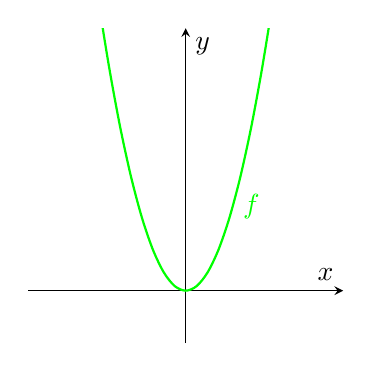
\begin{tikzpicture}\begin{axis}[
                xlabel=$x$,
                ylabel=$y$,
                axis equal,
                axis lines=middle,
                enlargelimits,
                xmax=5,
                xmin=-5,
                ymax=9,
                ymin=-1,
                xtick={0},
                ytick={0},
                scale only axis, 
                height=4cm, 
                width=4cm
                ]
            \addplot [no marks, green, smooth, thick, x=-1:5] {x^2};
            \node at (2.5, 3.2) {\textcolor{green}{$f$}};
        \end{axis}\end{tikzpicture}\end{center}
        \columnbreak

        \begin{center}
        \begin{tikzpicture}
            \begin{axis}[
                xlabel=$x$,
                ylabel=$y$,
                axis equal,
                axis lines=middle,
                enlargelimits,
                xmax=5,
                xmin=-1,
                ymax=5,
                ymin=-1,
                xtick={1},
                ytick={0},
                scale only axis, 
                height=4cm, 
                width=4cm
                ]
                \addplot [no marks, blue, smooth, thick, domain=0:5] {ln(x)};
                \node at (3, 1.7) {\textcolor{blue}{$g$}};
            \end{axis}
        \end{tikzpicture}\end{center}
    \end{multicols}

    Dal momento che $ f(D)=[0, + \infty) \nsubseteq D' $ non possiamo costruire $ g \circ f $. Restringiamo $ f $: \begin{align*}
    \tilde{f}:\R\setminus\{0\} & \to \R \\
    x & \mapsto x^{2}
    \end{align*} $ \tilde{f}(D)=(0,+ \infty) \subseteq\dom g $ \begin{align*}
    g\circ\tilde{f}:\R\setminus\{0\} & \to \R \\
    x & \mapsto \ln(x^{2})
    \end{align*}

    \begin{center}
        \begin{tikzpicture}
            \begin{axis}[
                xlabel=$x$,
                ylabel=$y$,
                axis equal,
                axis lines=middle,
                enlargelimits,
                xmax=5,
                xmin=-5,
                ymax=5,
                ymin=-1,
                xtick={0},
                ytick={0},
                scale only axis, 
                height=4cm, 
                width=6cm
                ]
                \addplot [no marks, red, unbounded coords=jump, thick] {ln(x^2)};
                \node at (1.4, 2.3) {\textcolor{red}{$\ln(x^{2})$}};
            \end{axis}
        \end{tikzpicture}\end{center}
}
\subsection{Funzione inversa}

Siano $ X, Y $ insiemi generici, $ D \subseteq X $. Se $ f:D\to Y $ è iniettiva, allora \[
    f:D\to f(D)
\] è \textit{biunivoca}, ovvero \begin{equation}
    \forall\,y \in f(D)\quad \exists!\, x \in D\quad y=f(x)
\end{equation}

Diciamo che $ f $ tra $ D $ e $ f(D) $ è \textit{invertibile}. Diciamo \textit{funzione inversa} di $ f $ \begin{align*}
\varphi:f(D) & \to D \\
y & \mapsto \varphi(y)=x
\end{align*} dove $ x $ è l'unico elemento di $ D $ tale che $ y=f(x) $. Si ha allora 
\[
    \begin{aligned}
        \varphi\circ f: D&\to D\\
        \dom f&\to \dom f\\
        x &\mapsto \varphi\circ f(x)=x
    \end{aligned}\hspace{4em}\begin{aligned}
        f\circ\varphi: f(D) &\to f(D)\\
        y&\mapsto f\circ\varphi(y)=y
    \end{aligned}
\] ossia \begin{equation}
    \varphi \circ f =\Id_{D} \qquad f\circ\varphi = \Id_{f(D)} 
\end{equation} dove $ \Id_{D}  $ è l'identità in $ D $ e $ \Id_{f(D)}  $ è l'identità in $ f(D) $.

La funzione inversa $ \varphi $ in genere si indica con $ f^{-1} $: \[
    f^{-1} \circ f =\Id_{D} \qquad f\circ f^{-1} = \Id_{f(D)}
\]
\esempio{}{
    \begin{align*}
    f:[0, + \infty) & \to [0, + \infty) \\
    x & \mapsto x^{2}
    \end{align*} $ \dom f =[0, + \infty) $: $ f  $ è biunivoca e dunque invertibile \begin{align*}
    f^{-1}:[0, + \infty) & \to [0, + \infty) \\
    x & \mapsto f^{-1}(x)= \sqrt{x}
    \end{align*}

    \begin{multicols}{2}
        \begin{center}\begin{tikzpicture}\begin{axis}[
                xlabel=$x$,
                ylabel=$y$,
                axis equal,
                axis lines=middle,
                enlargelimits,
                xmax=5,
                xmin=-5,
                ymax=9,
                ymin=-1,
                xtick={0},
                ytick={0},
                scale only axis, 
                height=4cm, 
                width=4cm
                ]
            \addplot [no marks, green, smooth, thick, domain=0:5] {x^2};
            \node at (2.5, 3.2) {\textcolor{green}{$f$}};
        \end{axis}\end{tikzpicture}\end{center}
        \columnbreak

        \begin{center}
        \begin{tikzpicture}
            \begin{axis}[
                xlabel=$x$,
                ylabel=$y$,
                axis equal,
                axis lines=middle,
                enlargelimits,
                xmax=5,
                xmin=-1,
                ymax=5,
                ymin=-1,
                xtick={0},
                ytick={0},
                scale only axis, 
                height=4cm, 
                width=4cm
                ]
                \addplot [no marks, blue, smooth, thick, domain=0:5] {x^0.5};
                \node at (1, 1.6) {\textcolor{blue}{$g$}};
            \end{axis}
        \end{tikzpicture}\end{center}
    \end{multicols}
    \begin{gather*}
        f^{-1}\circ f (x) = \sqrt{x^{2}}= x \qquad x\ge 0\\
        f \circ f^{-1}(x) = (\sqrt{x})^{2} = x\qquad x\ge 0
    \end{gather*}
}
\attenzione{
    Non confondere la funzione \textit{inversa} $ f^{-1} $ (ovvero tale che $f^{-1}\circ f =\id_{D} $) con la funzione \textit{reciproca} 
    \[
        [f(x)]^{-1}=\frac{1}{f(x)}
    \]
}

Nell'esempio precedente, funzione inversa e funzione reciproca sono ben diverse. Infatti, data \begin{align*}
f:[0,+ \infty) & \to [0, + \infty) \\
x & \mapsto x^{2}
\end{align*} vale che \[
    f^{-1}(x)=\sqrt{x}\qquad f(x)^{-1}=\frac{1}{x^{2}}
\] inoltre \[
    f \circ f^{-1}(x)=x\qquad f(x) \cdot f(x)^{-1}=1 \quad\forall\, x \in \R\setminus\{0\}
\]

\subsubsection{Grafico della funzione inversa}

\begin{center}
    \begin{tikzpicture}
        \begin{axis}[
            xlabel=$x$,
            ylabel=$y$,
            axis equal,
            axis lines=middle,
            enlargelimits,
            xmax=5,
            xmin=-1,
            ymax=5,
            ymin=-1,
            xtick={1},
            ytick={1},
            scale only axis, 
            height=7cm, 
            width=7cm,
            title={$f(x)=x^{2}\qquad x\ge 0$}
            ]
            \addplot [no marks, red, smooth, thick, domain=0:5] {x^0.5};
            \node at (4, 1.6) {\textcolor{red}{$f^{-1}(x)$}};
            \addplot [no marks, blue, smooth, thick, domain=0:5] {x^2};
            \node at (1.5, 4) {\textcolor{blue}{$f(x)$}};
            \addplot [no marks, green, dashed, thick] coordinates {(-3,-3) (7,7)};
        \end{axis}
    \end{tikzpicture}\end{center}

Il grafico di $ f^{-1} $ è il simmetrico del grafico di $ f $ rispetto alla bisettrice del primo e del terzo quadrante.

\esercizio{
    Verificare che la funzione $ f(x)=\sin x $ sia invertibile su $ \bigl[-\frac{\pi}{2}, +\frac{\pi}{2}\bigr] $, determinare il dominio dell'inversa e disegnare entrambi i grafici \[
        f^{-1}(x)=\arcsin x
    \]
}{
    Da risolvere %ESERCIZIO risolvere esercizio
}{}
\esercizio{
    Verificare che la funzione $ g(x)=\tan x $ è invertibile su $ \bigl(-\frac{\pi}{2}, +\frac{\pi}{2}\bigr) $, determinare dominio e grafico di $ g^{-1}(x) $ \[
        g^{-1}(x)=\arctan x
    \]
}{
    Da risolvere %ESERCIZIO risolvere esericizio
}{}

\subsection{Funzioni limitate}

Dato $ D \subseteq \R^{n} $,\begin{align*}
f:D & \to \R \\
x & \mapsto f(x)
\end{align*} è detta \textit{limitata} se $ f(D) $ è un insieme limitato, ossia \[
    \exists\, M>0\,\tc\quad \forall\, x \in D\qquad \begin{aligned}
        |f(x)|&<M\\
        -M<f(x)&< M
    \end{aligned}
\]

$ f $ è limitata superiormente (inferiormente) se \[
    \exists\, M>0\,\tc\quad \forall\, x \in D\qquad\begin{aligned}
        f(x)&<M\\
        \bigl(f(x)&>-M\bigr)
    \end{aligned}
\]

\esempio{}{
    \begin{align*}
    f:\R & \to \R \\
    x & \mapsto \sin x
    \end{align*} $ f $ è limitata in quanto $ f(D) \subseteq [-1, 1] $, ovvero \[
        \forall\, x \in \R\qquad -1\le f(x)\le 1
    \]
    \begin{center}
        \begin{tikzpicture}
            \begin{axis}[
                xlabel=$x$,
                ylabel=$y$,
                axis equal,
                axis lines=middle,
                enlargelimits,
                xmax=8,
                xmin=-8,
                ymax=2,
                ymin=-2,
                xtick={0},
                ytick={-1, 1},
                scale only axis, 
                height=4cm, 
                width=10cm]
                \addplot [no marks, blue, thick, samples=1000, domain=-8:8] {sin(x*180/3.1415)};
                \addplot [no marks, red, dashed, thick, domain=-8:8] {1};
                \addplot [no marks, red, dashed, thick, domain=-8:8] {-1};
            \end{axis}
        \end{tikzpicture}\end{center}
}
\definizione{}{
    Data $ f:D\to \R $, con $ D \subseteq \R $, diciamo \textit{estremo superiore} (inferiore) di $ f $ su $ D $ 
    \begin{align}
        \sup_{D} f &:= \sup\bigl(f(D)\bigr)\\
        \Bigl(\inf_{D} f &:= \inf\bigl(f(D)\bigr) \Bigr)
    \end{align} 
}
\esempio{Ecco due funzioni:

\begin{minipage}{\textwidth}
    \begin{multicols}{2}
        \begin{center}\begin{tikzpicture}\begin{axis}[
                xlabel=$x$,
                ylabel=$y$,
                axis equal,
                axis lines=middle,
                enlargelimits,
                xmax=5,
                xmin=-5,
                ymax=5,
                ymin=-5,
                xtick={0},
                ytick={0},
                scale only axis, 
                height=4cm, 
                width=4cm
                ]
            \addplot [no marks, green, smooth, thick, domain=-5:5] {x^3};
        \end{axis}\end{tikzpicture}\end{center} \begin{align*}
        f:\R & \to \R \\
        x & \mapsto x^{3}
        \end{align*}

        $ f $ non è limitata.
        \columnbreak

        \begin{center}
        \begin{tikzpicture}
            \begin{axis}[
                xlabel=$x$,
                ylabel=$y$,
                axis equal,
                axis lines=middle,
                enlargelimits,
                xmax=5,
                xmin=-1,
                ymax=5,
                ymin=-1,
                xtick={0},
                ytick={0},
                scale only axis, 
                height=4cm, 
                width=4cm
                ]
                \addplot [no marks, blue, smooth, thick, domain=0:5] {x^3};
\end{axis}\end{tikzpicture}\end{center}
\begin{align*}
g:[0,+\infty) & \to \R \\
x & \mapsto x^{3}
\end{align*} 

$ g $ è limitata inferiormente, e \[\inf_{[0,+ \infty)}  g =0=\min_{[0,+ \infty)}  g\]
\end{multicols}\end{minipage}}

\definizione{}{
    $ \sup f $ e $ \inf f$, se appartengono all'immagine $ f(D) $ sono detti \textit{valore massimo} e \textit{minimo} di $ f $.
}

\subsection{Massimi, minimi e monotonia}

Data $ f:D\to \R $, $ D \subseteq \R^{n} $, 
\begin{itemize}
\item $ x_0 \in D $ è \textit{punto di massimo} (\textit{minimo}) \textit{assoluto} o globale di $ f $ se \begin{equation}
    \forall\, x \in D\qquad \begin{aligned}
        f(x)&\le f(x_0)\\
        \bigl(f(x)&\ge f(x_0)\bigr)
    \end{aligned}
\end{equation}
\item $ x_0 $ è detto \textit{punto di massimo} (\textit{minimo}) \textit{locale} o relativo di $ f $ se \begin{equation}
    \exists\, U(x_0)\,\tc\quad \forall\, x \in U(x_0)\quad \begin{aligned}
        f(x)&\le f(x_0)\\
        \bigl(f(x)&\ge f(x_0)\bigr)
    \end{aligned}
\end{equation}
\item $ x_0 $ è detto \textit{punto di massimo} (\textit{minimo}) \textit{forte} di $ f $ se \begin{equation}
    \begin{aligned}
        \forall\, x &\in D\\
        \bigl(\exists\, U(x_0)\,\tc\quad \forall\, x &\in U(x_0)\bigr)
    \end{aligned}\qquad
     x\neq x_0\text{ si ha}\quad \begin{aligned}
        f(x)&< f(x_0)\\
        \bigl(f(x)&> f(x_0)\bigr)
    \end{aligned}
\end{equation}
\end{itemize}

\subsubsection{Funzioni monotone}   

Data $ f:D\to \R $, $ D \subseteq \R^{n} $, 
\begin{itemize}
\item $ f $ è \textit{crescente} (\textit{decrescente}) su $D $ se \begin{equation}
    \forall\, x_1, x_2 \in D\qquad x_1<x_2 \,\implies\, \begin{aligned}
        f(x_1)&\le f(x_2)\\
        \bigl(f(x_1)&\ge f(x_2)\bigr)
    \end{aligned}
\end{equation}
\item $ f $ è \textbf{strettamente} \textit{crescente} (\textit{decrescente}) su $D $ se \begin{equation}
    \forall\, x_1, x_2 \in D\qquad x_1<x_2 \,\implies\, \begin{aligned}
        f(x_1)&< f(x_2)\\
        \bigl(f(x_1)&> f(x_2)\bigr)
    \end{aligned}\end{equation}
\end{itemize}